%!TEX root = ../../Algorithms.tex
\documentclass[Chapter02]{subfiles}

\tikzset{
	sort node/.style = {
		rectangle,
		draw = black,
		anchor = north west
	},
	curs node/.style = {
		sort node,
		text = white,
		fill = black
	},
	comp node/.style = {
		sort node,
		fill = gray
	}
}

\begin{document}
	\subsection{Insertion Sort}

	\begin{enumerate}[leftmargin=\labelsep]
		% 2.1-1
		\item Using Figure 2.2 as a model, illustrate the operation of \textsc{Insertion-Sort} on the array $A = \langle 31, 41, 59, 26, 41, 58 \rangle$.
		\begin{figure}[ht]
			\floatsetup{valign=t, heightadjust=object, capposition=top}
			\begin{subfloatrow}[3]
				\centering
				\floatbox{figure}{\caption{}}{
					\tikzsetnextfilename{Chapter02-insertion-sort-01}
					\scalebox{1.5}{
						\begin{tikzpicture}
							\node at (0,0)          [comp node, label={\tiny 1}] (a) {5};
							\node at (a.north east) [curs node, label={\tiny 2}] (b) {2};
							\node at (b.north east) [sort node, label={\tiny 3}] (c) {4};
							\node at (c.north east) [sort node, label={\tiny 4}] (d) {6};
							\node at (d.north east) [sort node, label={\tiny 5}] (e) {1};
							\node at (e.north east) [sort node, label={\tiny 6}] (f) {3};

							\draw [-{Stealth[length=1mm]}, gray] (a.290) to[out=270, in=270, looseness=2] (b.250);
							\draw [-{Stealth[length=1mm]}]       (b.300) to[out=270, in=270, looseness=2] (a.240);
						\end{tikzpicture}
					}
				}
				\floatbox{figure}{\caption{}}{
					\tikzsetnextfilename{Chapter02-insertion-sort-02}
					\scalebox{1.5}{
						\begin{tikzpicture}
							\node at (0,0)          [comp node, label={\tiny 1}] (a) {2};
							\node at (a.north east) [comp node, label={\tiny 2}] (b) {5};
							\node at (b.north east) [curs node, label={\tiny 3}] (c) {4};
							\node at (c.north east) [sort node, label={\tiny 4}] (d) {6};
							\node at (d.north east) [sort node, label={\tiny 5}] (e) {1};
							\node at (e.north east) [sort node, label={\tiny 6}] (f) {3};

							\draw [-{Stealth[length=1mm]}, gray] (b.290) to[out=270, in=270, looseness=2] (c.250);
							\draw [-{Stealth[length=1mm]}]       (c.300) to[out=270, in=270, looseness=2] (b.240);
						\end{tikzpicture}
					}
				}
				\floatbox{figure}{\caption{}}{
					\tikzsetnextfilename{Chapter02-insertion-sort-03}
					\scalebox{1.5}{
						\begin{tikzpicture}
							\node at (0,0)          [sort node, label={\tiny 1}] (a) {2};
							\node at (a.north east) [sort node, label={\tiny 2}] (b) {4};
							\node at (b.north east) [comp node, label={\tiny 3}] (c) {5};
							\node at (c.north east) [curs node, label={\tiny 4}] (d) {6};
							\node at (d.north east) [sort node, label={\tiny 5}] (e) {1};
							\node at (e.north east) [sort node, label={\tiny 6}] (f) {3};

							\draw [-{Stealth[length=1mm]}] (d.300) to[out=270, in=270, looseness=4] (d.240);
						\end{tikzpicture}
					}
				}
			\end{subfloatrow}
			\begin{subfloatrow}[3]
				\centering
				\floatbox{figure}{\caption{}}{
					\tikzsetnextfilename{Chapter02-insertion-sort-04}
					\scalebox{1.5}{
						\begin{tikzpicture}
							\node at (0,0)          [comp node, label={\tiny 1}] (a) {2};
							\node at (a.north east) [comp node, label={\tiny 2}] (b) {4};
							\node at (b.north east) [comp node, label={\tiny 3}] (c) {5};
							\node at (c.north east) [comp node, label={\tiny 4}] (d) {6};
							\node at (d.north east) [curs node, label={\tiny 5}] (e) {1};
							\node at (e.north east) [sort node, label={\tiny 6}] (f) {3};

							\draw [-{Stealth[length=1mm]}, gray] (a.290) to[out=270, in=270, looseness=2] (b.250);
							\draw [-{Stealth[length=1mm]}, gray] (b.290) to[out=270, in=270, looseness=2] (c.250);
							\draw [-{Stealth[length=1mm]}, gray] (c.290) to[out=270, in=270, looseness=2] (d.250);
							\draw [-{Stealth[length=1mm]}, gray] (d.290) to[out=270, in=270, looseness=2] (e.250);
							\draw [-{Stealth[length=1mm]}, rounded corners=.3cm]   (e.300) -- +(0,-.4) -| (a.240);
						\end{tikzpicture}
					}
				}
				\floatbox{figure}{\caption{}}{
					\tikzsetnextfilename{Chapter02-insertion-sort-05}
					\scalebox{1.5}{
						\begin{tikzpicture}
							\node at (0,0)          [sort node, label={\tiny 1}] (a) {1};
							\node at (a.north east) [comp node, label={\tiny 2}] (b) {2};
							\node at (b.north east) [comp node, label={\tiny 3}] (c) {4};
							\node at (c.north east) [comp node, label={\tiny 4}] (d) {5};
							\node at (d.north east) [comp node, label={\tiny 5}] (e) {6};
							\node at (e.north east) [curs node, label={\tiny 6}] (f) {3};

							\draw [-{Stealth[length=1mm]}, gray] (c.290) to[out=270, in=270, looseness=2] (d.250);
							\draw [-{Stealth[length=1mm]}, gray] (d.290) to[out=270, in=270, looseness=2] (e.250);
							\draw [-{Stealth[length=1mm]}, gray] (e.290) to[out=270, in=270, looseness=2] (f.250);
							\draw [-{Stealth[length=1mm]}, rounded corners=.3cm]   (f.300) -- +(0,-.4) -| (c.240);
						\end{tikzpicture}
					}
				}
				\floatbox{figure}{\caption{}}{
					\tikzsetnextfilename{Chapter02-insertion-sort-06}
					\scalebox{1.5}{
						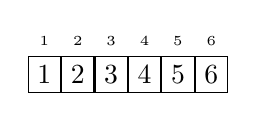
\begin{tikzpicture}
							\node at (0,0)          [sort node, label={\tiny 1}] (a) {1};
							\node at (a.north east) [sort node, label={\tiny 2}] (b) {2};
							\node at (b.north east) [sort node, label={\tiny 3}] (c) {3};
							\node at (c.north east) [sort node, label={\tiny 4}] (d) {4};
							\node at (d.north east) [sort node, label={\tiny 5}] (e) {5};
							\node at (e.north east) [sort node, label={\tiny 6}] (f) {6};
						\end{tikzpicture}
					}
				}
			\end{subfloatrow}
		\end{figure}
		\begin{answer}
			\hfill\\
			\begin{figure}[ht]
				\floatsetup{valign=t, heightadjust=object, style=plaintop}
				\begin{subfloatrow}[3]
					\centering
					\floatbox{figure}{\caption{}}{
						\tikzsetnextfilename{Chapter02-insertion-sort-answer-01}
						\scalebox{1.5}{
							\begin{tikzpicture}
								\node at (0,0)          [comp node, label={\tiny 1}] (a) {31};
								\node at (a.north east) [curs node, label={\tiny 2}] (b) {41};
								\node at (b.north east) [sort node, label={\tiny 3}] (c) {59};
								\node at (c.north east) [sort node, label={\tiny 4}] (d) {26};
								\node at (d.north east) [sort node, label={\tiny 5}] (e) {41};
								\node at (e.north east) [sort node, label={\tiny 6}] (f) {58};

								\draw [-{Stealth[length=1mm]}] (b.300) to[out=270, in=270, looseness=4] (b.240);
							\end{tikzpicture}
						}
					}

					\floatbox{figure}{\caption{}}{
						\tikzsetnextfilename{Chapter02-insertion-sort-answer-02}
						\scalebox{1.5}{
							\begin{tikzpicture}
								\node at (0,0)          [sort node, label={\tiny 1}] (a) {31};
								\node at (a.north east) [comp node, label={\tiny 2}] (b) {41};
								\node at (b.north east) [curs node, label={\tiny 3}] (c) {59};
								\node at (c.north east) [sort node, label={\tiny 4}] (d) {26};
								\node at (d.north east) [sort node, label={\tiny 5}] (e) {41};
								\node at (e.north east) [sort node, label={\tiny 6}] (f) {58};

								\draw [-{Stealth[length=1mm]}] (c.300) to[out=270, in=270, looseness=4] (c.240);
							\end{tikzpicture}
						}
					}

					\floatbox{figure}{\caption{}}{
						\tikzsetnextfilename{Chapter02-insertion-sort-answer-03}
						\scalebox{1.5}{
							\begin{tikzpicture}
								\node at (0,0)          [comp node, label={\tiny 1}] (a) {31};
								\node at (a.north east) [comp node, label={\tiny 2}] (b) {41};
								\node at (b.north east) [comp node, label={\tiny 3}] (c) {59};
								\node at (c.north east) [curs node, label={\tiny 4}] (d) {26};
								\node at (d.north east) [sort node, label={\tiny 5}] (e) {41};
								\node at (e.north east) [sort node, label={\tiny 6}] (f) {58};

								\draw [-{Stealth[length=1mm]}, gray] (a.290) to[out=270, in=270, looseness=2] (b.250);
								\draw [-{Stealth[length=1mm]}, gray] (b.290) to[out=270, in=270, looseness=2] (c.250);
								\draw [-{Stealth[length=1mm]}, gray] (c.290) to[out=270, in=270, looseness=2] (d.250);
								\draw [-{Stealth[length=1mm]}, rounded corners=.3cm]   (d.300) -- +(0,-.4) -| (a.240);
							\end{tikzpicture}
						}
					}
				\end{subfloatrow}
			\end{figure}
		\end{answer}

		% 2.1-2
		\item Rewrite the \textsc{Insertion-Sort} procedure to sort into nonincreasing instead of nondecreasing order.
		\begin{answer}
			
		\end{answer}

		% 2.1-3
		\item Consider the \textbf{\textit{searching problem}}:\\[.5em]
		\textbf{Input:} A sequence of $n$ number $A = \langle a_1, a_2, \dots, a_n \rangle$ and a value $v$.\\[.5em]
		\textbf{Output:} An index $i$ such that $v = A[i]$ or the special value \texttt{NIL} if $v$ does not appear in $A$.\\[.5em]
		Write pseudocode for \textbf{\textit{linear-search}}, which scans through the sequence, looking for $v$. using a loop invariant, prove that your algorithm is correct. Make sure that your loop invariant fulfills the three necessary properties.
		\begin{answer}
			
		\end{answer}

		% 2.1-4
		\item Consider the problem of adding two $n$-bit binary integers, stored in two $n$-element arrays $A$ and $B$, The sum of the two integers should be stored in binary form in an $(n + 1)$-element array $C$. State the problem formally and write pseudocode for adding the two integers.
		\begin{answer}
			
		\end{answer}
	\end{enumerate}

\end{document}